\chapter{Конструкторский раздел}
\label{cha:design}

\section{Модель}
\begin{figure}
    \centering
    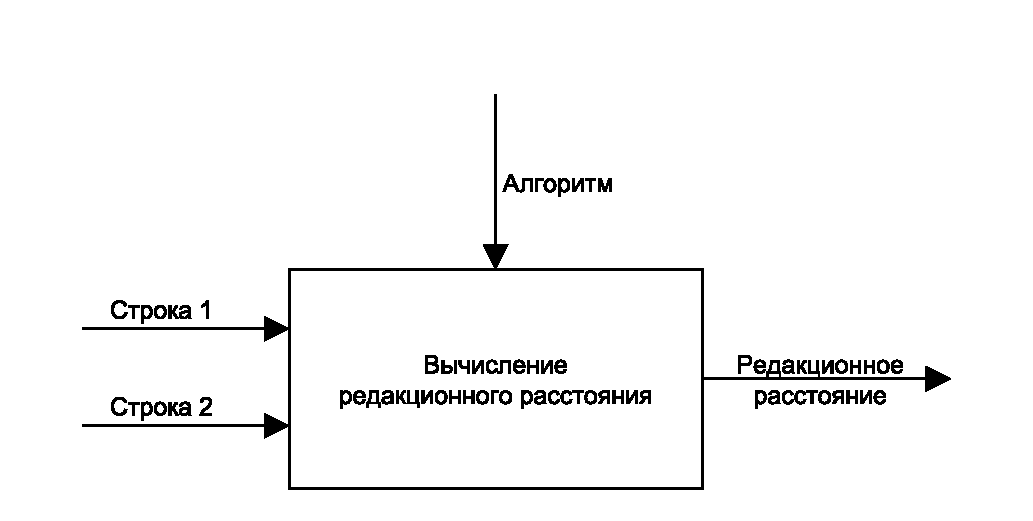
\includegraphics{pdf/mainIdef0.pdf}
    \caption{IDEF\O{} модель}
\end{figure}

\section{Разработка алгоритмов}

\subsection{Алгоритм Вагнера-Фишера}
Алгоритм Вагнера-Фишера является матричной реализацией поиска расстояния Левенштейна. Ниже приведена блок-схема данного алгоритма.
\begin{figure}
    \centering
    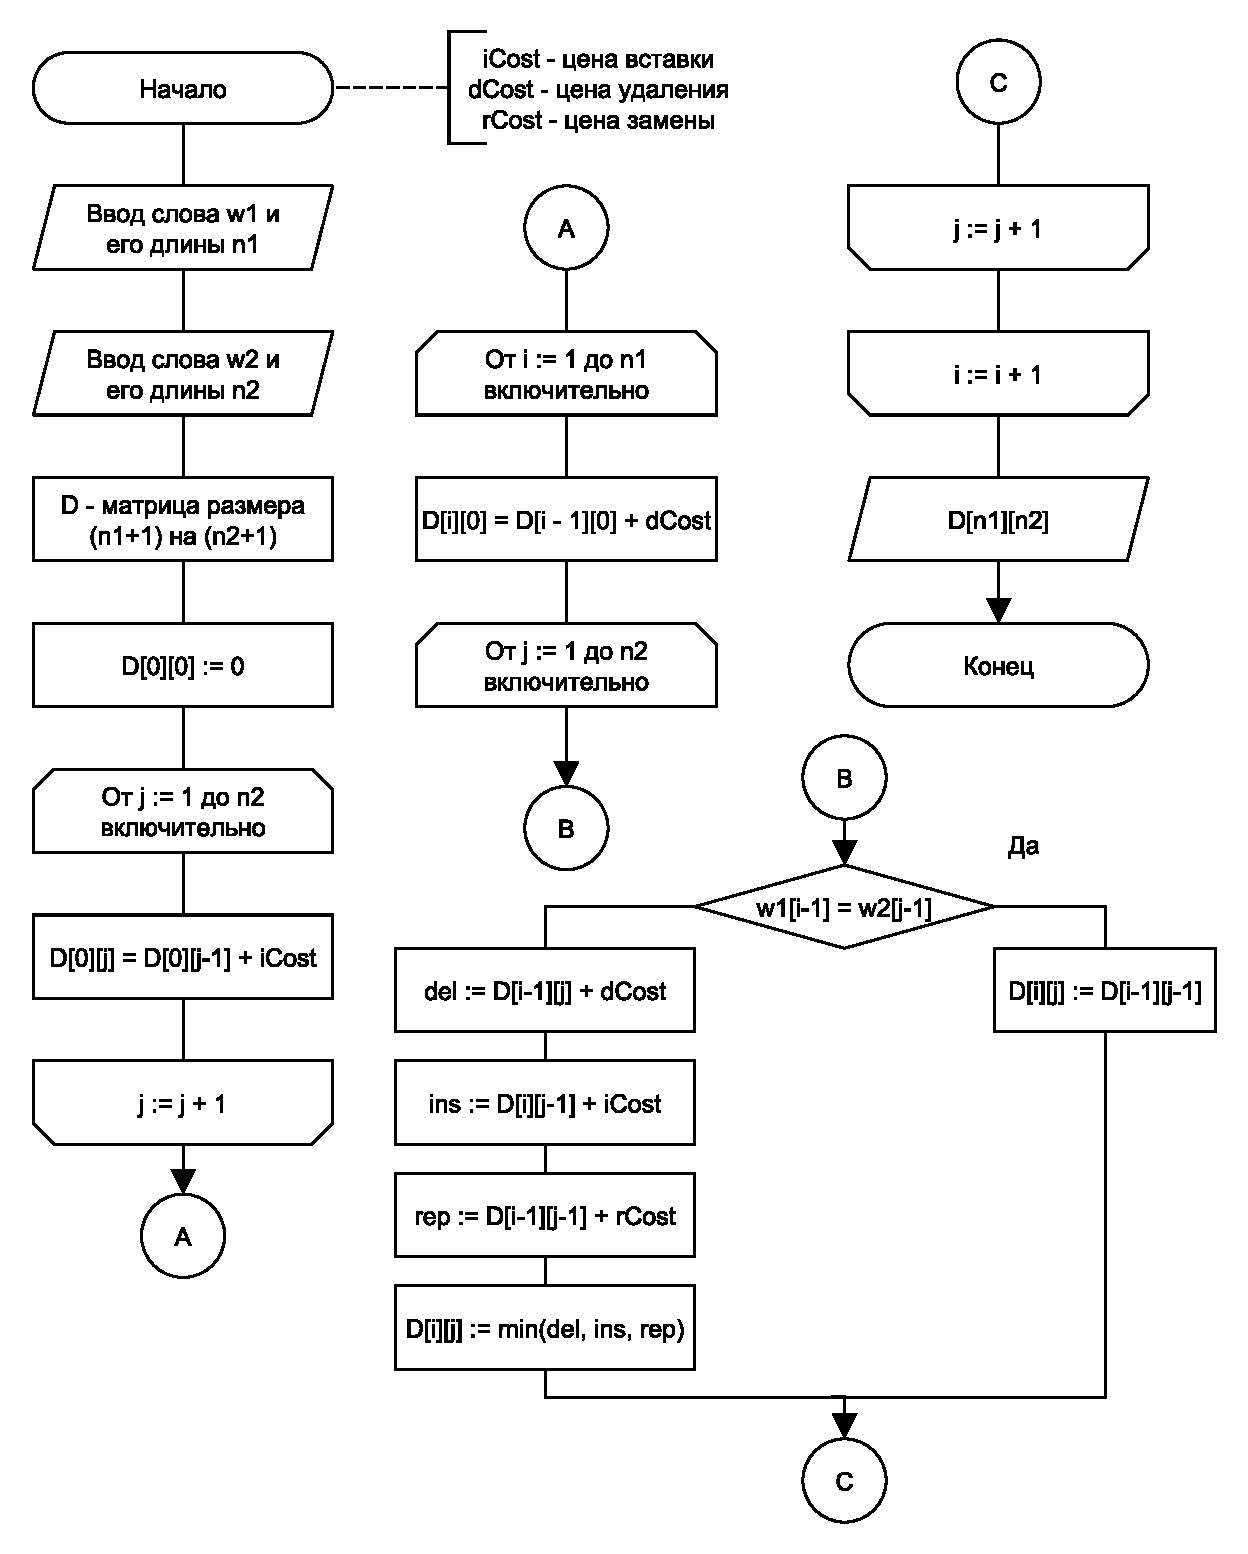
\includegraphics[scale=0.8]{pdf/wagner-fischer-all.pdf}
    \caption{Алгоритм Вагнера-Фишера}
\end{figure}

\newpage
\subsection{Матричный алгоритм Дамерау-Левенштейна}

